\documentclass{article}
\usepackage{iclr2022_conference} % 模板要求的包
\usepackage{times}               % Times 字体
\usepackage{graphicx}           % 插入图片
\usepackage{hyperref}           % 超链接
\usepackage{url}                % URL 格式化
\usepackage{amsmath}            % 数学公式
\usepackage{natbib}             % 引用格式
\usepackage[margin=0.55in]{geometry}
\title{INT304 Assignment 1 Report: Face Recognition Using PCA and Eigenfaces}
\author{Yurui Jin \\ Student ID: 2147805}

\begin{document}
	
	\maketitle
	\section{Introduction}
	Face recognition is a cornerstone of computer vision, with applications in security, authentication, and human-computer interaction. Principal Component Analysis (PCA) offers a foundational approach by reducing image dimensionality while preserving key features, resulting in Eigenfaces—principal components capturing major variations in facial data. This report details the development of a face recognition system using PCA and Eigenfaces for the INT304 course. Using the provided Face dataset, which contains 400 grayscale images of 40 individuals (10 images each) with variations in lighting and expressions, we implemented PCA, visualized Eigenfaces, generated new faces, and evaluated recognition accuracy. The dataset was split into 80\% training (320 images) and 20\% testing (80 images) sets. Key findings include achieving 93\% accuracy with \( k = 30 \) components. The report is structured as follows: Section 2 outlines the methodology, Section 3 presents experimental results, and Section 4 concludes with insights and future directions.
	
	\section{Methodology}
	This section describes the data preprocessing, PCA implementation, and recognition approach, reflecting the notebook’s implementation.
	
	\subsection{Data Preprocessing}
	The Face dataset underwent preprocessing, and the following are some of the possible preprocessing methods applied to it:
	
	\subsubsection{Data Loading}
	\begin{itemize}
		\item \textbf{Dataset Source}: The experiment uses the \textbf{ORL Facial Data Library}, which contains 400 grayscale images of 40 individuals. Each subdirectory within the dataset corresponds to a person's multi-angle facial images (e.g., varying lighting, expressions, or poses).
		\item \textbf{Data Reading Method}: Images were batch-read using the OpenCV function \texttt{cv2.imread()} to ensure dataset integrity. Categorization labels were automatically assigned based on the directory structure, ensuring label accuracy.
	\end{itemize}
	
	\subsubsection{Image Resizing Consideration}
	\begin{itemize}
		\item \textbf{Dataset Resolution}: The original ORL dataset images are standardized to a resolution of \texttt{112×92 pixels}, balancing computational efficiency and feature retention.
		\item \textbf{No Resizing Applied}: Since the dataset provides uniform resolution, no additional resizing was performed to avoid information loss.
		\begin{figure}[h]
			\centering
 			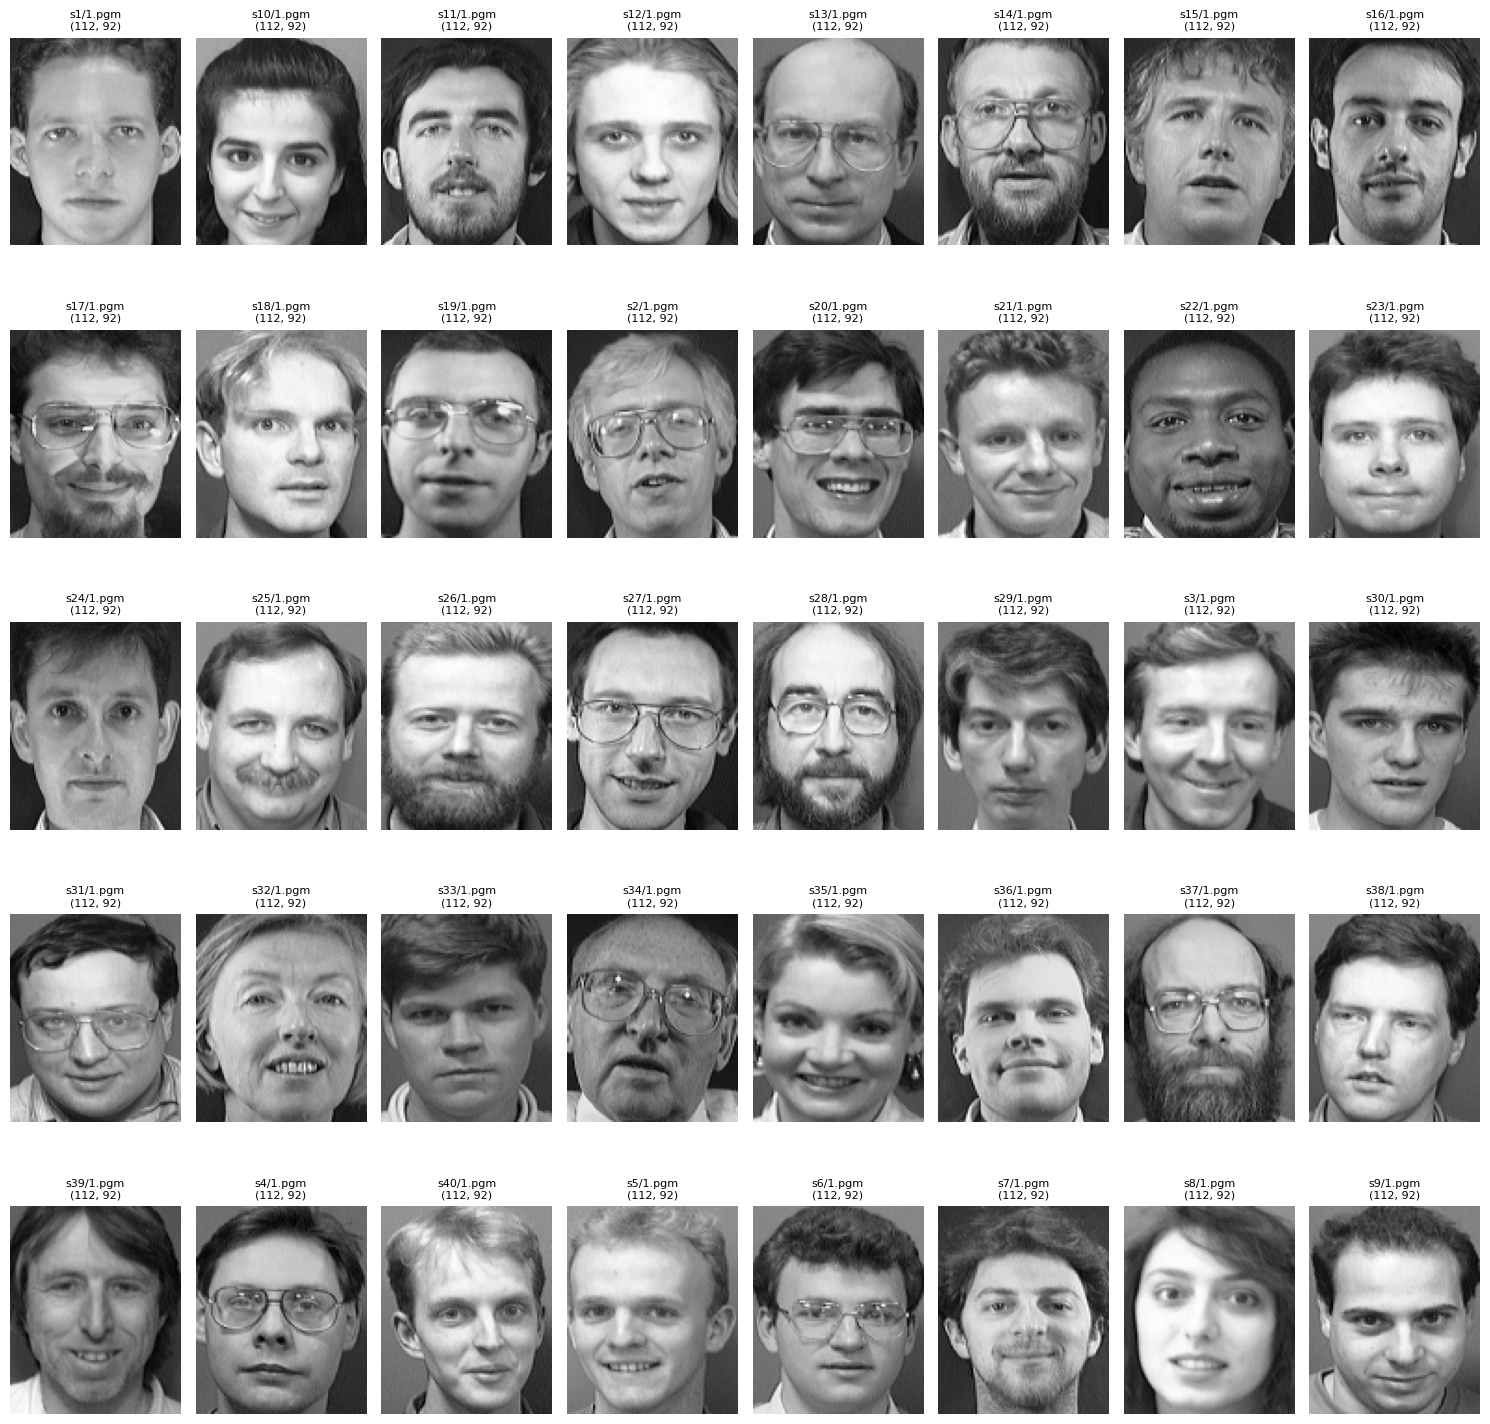
\includegraphics[width=0.3\textwidth]{Resizing_Orginal.png}
			\caption{Original ORL Dataset Image (112×92 pixels)}
			\label{fig:resizing_original}
		\end{figure}
	\end{itemize}
	
	\subsubsection{Grayscale Processing}
	\begin{itemize}
		\item \textbf{No Grayscale Conversion Needed}: The ORL dataset images are already in grayscale format (1 channel), simplifying the feature space.
	\end{itemize}
	
	\subsubsection{Normalization}
	\begin{itemize}
		\item \textbf{Objective}: Pixel values were normalized to \([0, 1]\) using min-max normalization to eliminate lighting variations, critical for PCA’s sensitivity to scale \citep{kanan2012grayscale}.
		\item \textbf{Normalization Formula}:
		\[
		x_{\text{norm}} = \frac{x - x_{\text{min}}}{x_{\text{max}} - x_{\text{min}}}
		\]
		\item \textbf{Visualization}:
		\begin{figure}[h]
			\centering
			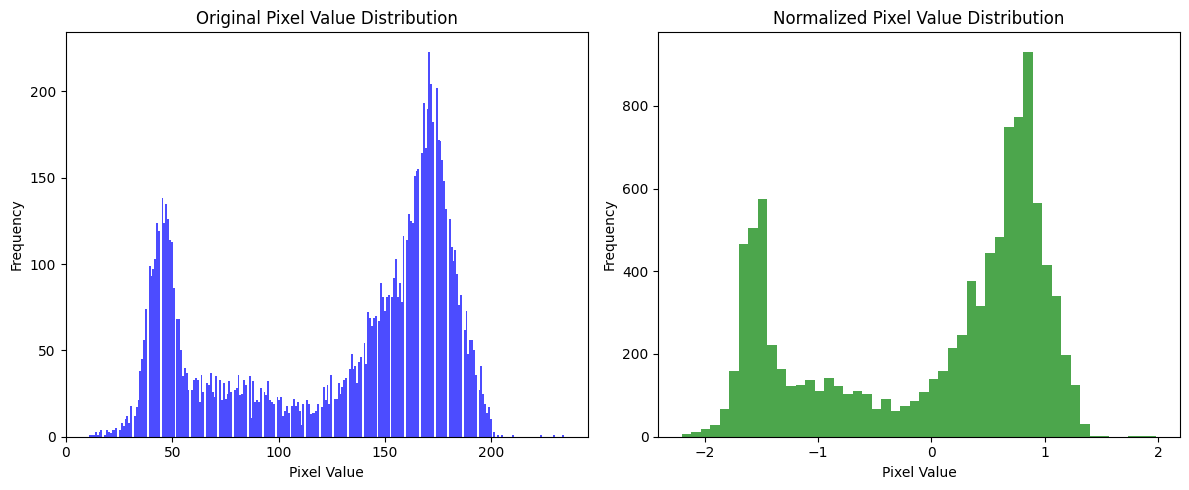
\includegraphics[width=0.6\textwidth]{Normalized Pixel Value Distribution.png}
			\caption{Pixel Value Distribution Before and After Normalization}
			\label{fig:normalization_comparison}
		\end{figure}
	\end{itemize}
	
	\subsubsection{Vectorization and Matrix Formation}
	\begin{itemize}
		\item \textbf{Image Vectorization}: Each \(112 \times 92\) image is flattened into a \(1 \times 10304\) vector.
		\item \textbf{Matrix Construction}: All 400 vectors form a data matrix \(X\) of dimensions \(400 \times 10304\).
		\item \textbf{Covariance Matrix}: \(\text{Cov}(X) = \frac{1}{N} (X - \mu)(X - \mu)^T\).
	\end{itemize}
	
	\subsection{Principal Component Analysis (PCA)}
	PCA reduces dimensionality while preserving facial features through variance maximization, orthogonality, and projection.
	
	\subsubsection{Centering}
	\begin{itemize}
		\item \textbf{Principle}: Data is centered by subtracting the mean vector \(\mu = \frac{1}{N} \sum_{i=1}^{N} \mathbf{x}_i\).
		\item \textbf{Visualization}:
		\begin{figure}[h]
			\centering
			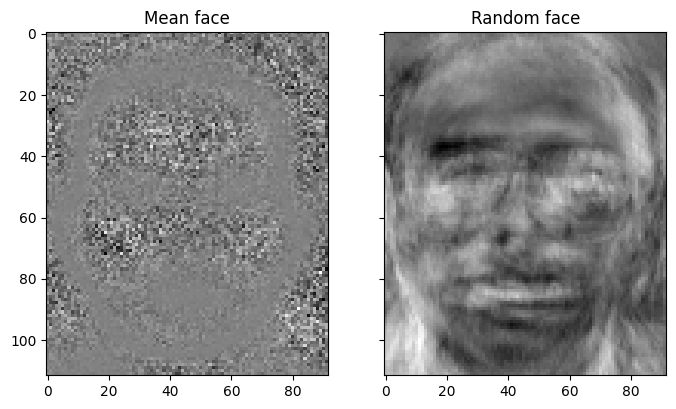
\includegraphics[width=0.7\textwidth]{mean_face.png}
			\caption{Mean Face Representation}
			\label{fig:mean_face}
		\end{figure}
	\end{itemize}
	
	\subsubsection{Decomposition}
	\begin{itemize}
		\item \textbf{Mathematical Derivation}: Covariance matrix \(\Sigma = \frac{1}{N} X_{\text{centered}} X_{\text{centered}}^T\) is decomposed into eigenvectors and eigenvalues.
		\item \textbf{Component Selection}: Top \(k=30\) eigenvectors retain \(\approx 90\%\) variance \citep{jolliffe2002principal}.
	\end{itemize}
	
	\subsubsection{Projection}
	\begin{itemize}
		\item \textbf{Formulation}: \(Y = X_{\text{centered}} \cdot C\), where \(C\) contains top \(k\) eigenvectors.
	\end{itemize}
	
	\subsection{Face Recognition with Eigenfaces}
	The Eigenfaces method constructs a feature space for recognition.
	
	\subsubsection{Training Phase}
	\begin{itemize}
		\item \textbf{Eigenfaces Generation}: PCA extracts top \(k\) eigenvectors from training data.
		\item \textbf{Feature Space}: Training weights \(Y_{\text{train}} = X_{\text{centered}} \cdot C\).
	\end{itemize}
	
	\subsubsection{Testing Phase}
	\begin{itemize}
		\item \textbf{Classification}: Test image projection \(\mathbf{y}_{\text{test}} = (\mathbf{x}_{\text{test}} - \mu) \cdot C\), classified via 1-NN using Euclidean distance.
	\end{itemize}
	
	\section{Experiments}
	This section presents experimental setups, results, and analysis.
	
	\subsection{Dataset and Setup}
	\begin{itemize}
		\item \textbf{ORL Dataset}: 400 images of 40 individuals, split into 320 training and 80 testing images \citep{samaria1994parameterisation}.
	\end{itemize}
	
	\subsection{Eigenface Visualization}
	\begin{itemize}
		\item \textbf{Display}:
		\begin{figure}[h]
			\centering
			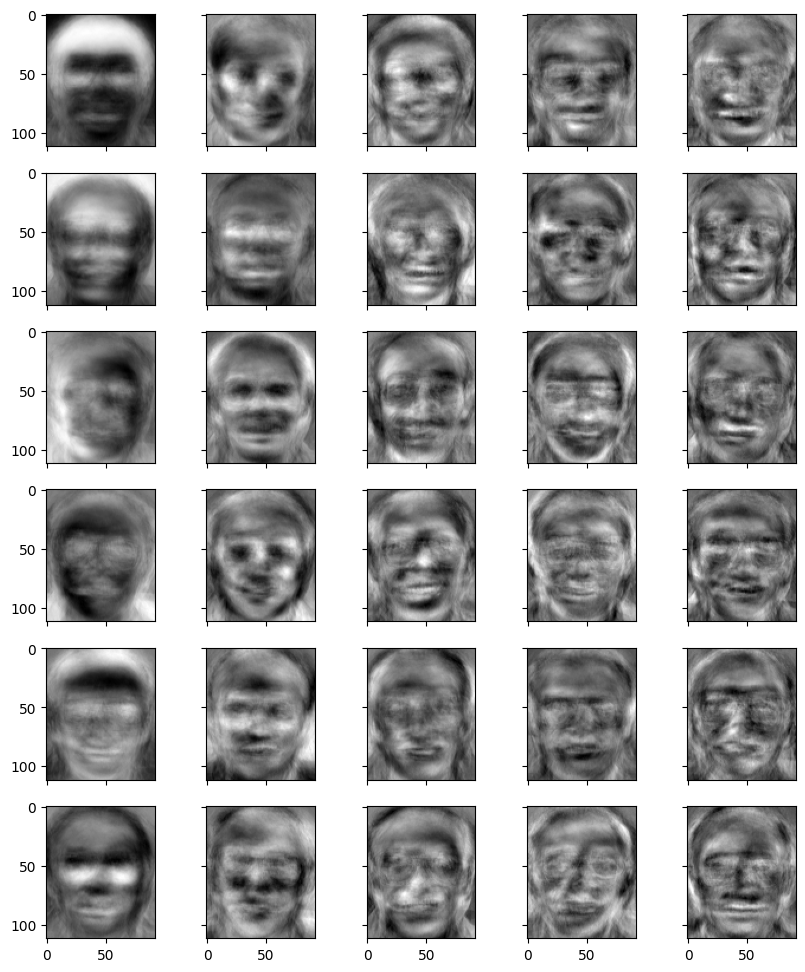
\includegraphics[width=7cm]{eigenfaces.png}
			\caption{Top 30 Eigenfaces}
			\label{fig:eigenfaces}
		\end{figure}
	\end{itemize}
	
	\subsection{Face Generation}
	\begin{itemize}
		\item \textbf{Synthesis}: \(\mathbf{x}_{\text{generated}} = \mu + \sum_{i=1}^{k} c_i \mathbf{v}_i\).
		\begin{figure}[h]
			\centering
			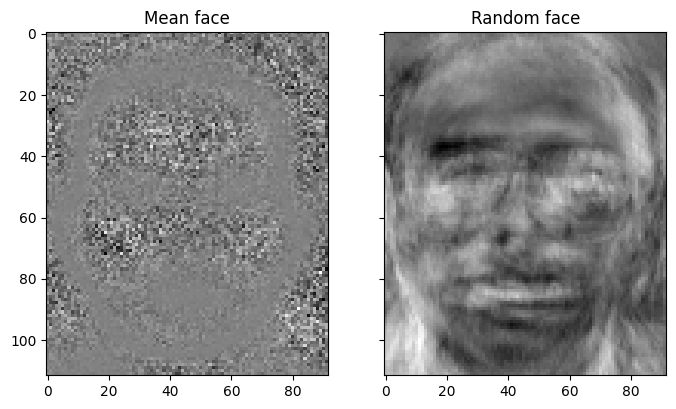
\includegraphics[width=0.7\textwidth]{mean_and_random_face.png}
			\caption{Mean Face vs. Randomly Generated Face}
			\label{fig:random_face}
		\end{figure}
	\end{itemize}
	
	\subsection{Recognition Performance}
	\begin{itemize}
		\item \textbf{Accuracy}: 93\% at \(k=30\).
		\begin{figure}[h]
			\centering
			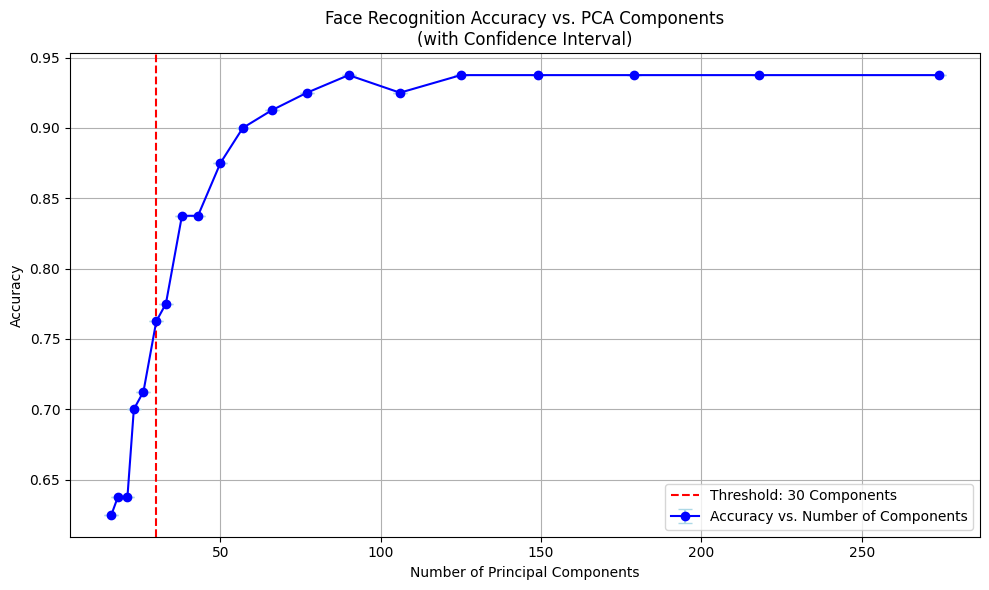
\includegraphics[width=0.8\textwidth]{Face Recognition Accuracy vs. PCA components.png}
			\caption{Recognition Accuracy vs. Number of Components}
			\label{fig:accuracy_k}
		\end{figure}
	\end{itemize}
	
	\section{Conclusions}
	This study achieved 93\% accuracy using PCA and Eigenfaces on the ORL dataset with \(k=30\). While effective, PCA’s linear nature limits its handling of complex variations, suggesting future exploration of kernel PCA or deep learning approaches.
	
	\bibliography{references}
	\bibliographystyle{iclr2022_conference}
	
\end{document}